 \subsection{Universidad de Mosku - Rusia}
Presentamos en la siguiente tabla los resultados obtenidos del último monitoreo.

\bigskip

\begin{tabular}{| l | c | c | c | c |}
 \hline 
Hop & IP &  RTT promedio (s)  & deltaRTT promedio & Ubicación\\
\hline 
1  &  192.168.0.1  &  0.00328697348541    &  0.00328697348541 & Argentina\\
\hline 
2  &  200.89.164.165  &  0.0182673031429    &  0.0149803296575 & Argentina\\
\hline 
3  &  200.89.165.130  &  0.018018808005    &  0 & Argentina\\
\hline 
4  &  200.89.165.222  &  0.023129620642   &  0.00511081263704 & Argentina\\
\hline 
5  &  206.165.31.213  &  0.0159362801966    &  0 & United States\\ 
\hline 
6  &  67.17.75.66  &  0.153266360362    &  0.137330080166 &  United States\\
\hline 
7  &  4.68.111.121  &  0.144784176125    &  0 & United States\\ 
\hline 
8  &  4.69.158.253  &  0.267091494686    &  0.122307318561 &  United States\\
\hline 
9  &  4.69.158.253  &  0.266443899045    &  0 & United States\\
\hline 
10  &  213.242.110.198  &  0.313186002227    &  0.0467421031829 & United Kingdom\\
\hline 
11  &  194.85.40.229  &  0.313147967716    &  0 & Russian Federation\\
\hline 
12  &  194.190.254.118  &  0.295875315396    &  0 & Russian Federation\\
\hline 
13  &  93.180.0.172  &  0.310500500249   &  0.0146251848526 & Moscow City Russian Federation\\
\hline 
14  &  188.44.33.30  &  0.293746012562    &  0 & Moscow City\\
\hline 
15  &  188.44.50.103  &  0.286035416261   &  0 & Moscow City\\
\hline 
\end{tabular}

De manera preliminar puede verse que la diferencia temporal entre los diferentes hops permanece en el orden de los $10^-3$ segundos, 
habiendo tan solo dos casos en que esto no sucede. Primero en el salto $6$ y luego en el salto $8$ que se encuentran en el orden de los $10^-1$ 
segundos.

A continuación se muestra el grafico de los RTT en cada hop, donde puede verse de manera visual que los saltos temporales mas abruptos se dan en 
el 6 y en el 8:

\bigskip

\begin{figure}[H]
\centering
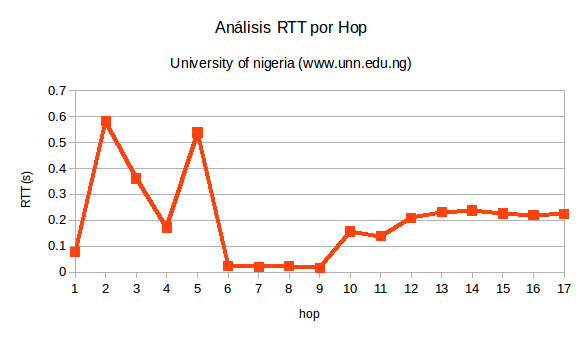
\includegraphics[width=1\textwidth]{graficos/zScore_rus.png}
\caption{zScore promedio por hop - Universidad de Mosku}
\label{Rus_zs}
\end{figure}

En este momento realizamos el test de hipotesis para ver si podemos aproximar los reslutados de los delta rtt a una distribución normal. 
El test de hipotesis que podemos aceptar la hipotesis con una confianza de $0.995$

Por lo tanto calculamos los zScore donde podremos apreciar cuan alejados estan los valores de la media y los graficamos:

\begin{figure}[H]
\centering
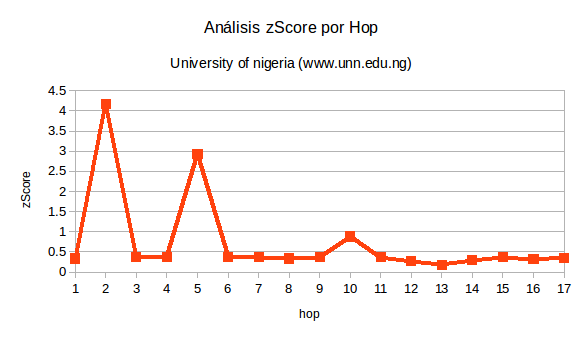
\includegraphics[width=1\textwidth]{graficos/RTT_rus.png}
\caption{RTT promedio por hop - Universidad de Mosku}
\label{Rus_rtt}
\end{figure}

Aqui tambien puede verse que los valores 6 y 8 son los mas patologicos y por lo tanto, los mejores candidatos a ser enlaces submarinos.

Finalmente utilizando el test de grubbs, obtenemos que efectivamente estos valores son outliers dentro de esta distribución normal, y por lo tanto, los saltos que mas probablemente correspondan a saltos submarinos.

Aun asi resulta extraño ver que tanto en el hop 6 como en el 8 las ips dicen estar asignadas a estados unidos. Esto podría deberse a que aunque las ips esten asignadas a estados unidos, el lugar fisico donde se encuentren sea otro.

Utilizando la herramienta http://www.infobyip.com/ pudimos observar algunos de los nombres de los hosts por los cuales hicimos el traceroute.

De esto conseguimos la siguiente tabla:

\begin{tabular}{| l | c | c }
\hline 
hop & IP & Host name\\
\hline 
5  &  206.165.31.213  &  xe-8-3-0.ar3.eze1.gblx.net\\
\hline 
6  &  67.17.75.66  &   po3-20G.ar3.MIA2.gblx.net\\
\hline 
7  &  4.68.111.121  & ae5.edge2.miami2.level3.net\\
\hline 
8  &  4.69.158.253  & ae-114-3504.bar1.Stockholm1.Level3.net\\
\end{tabular}

Tomando como hipotesis que los nombres de los hosts se correspondan con su hubicación geografica, entonces nuestros resultados sobre 
cuales son los saltos submarinos parecerían tener sentido ya que del salto 5 al salto 6 el paquete habría viajado desde argentina hasta miami y 
del salto 7 al salto 8 el paquete pareceria haber viajado de miami a estocolmo.

A continuación hemos trazado en un mapa la ruta de nuestro host hasta el host destino ubicado en Rusia:
\begin{figure}[H]
\centering
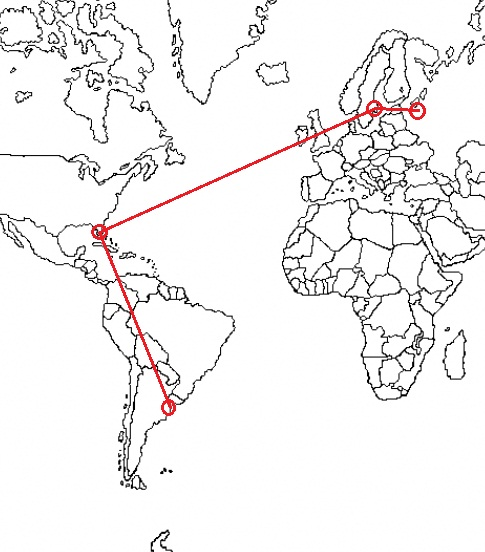
\includegraphics[width=0.8\textwidth]{graficos/mapa_rusia.jpg}
\caption{Ruta en Internet - Universidad de Mosku}
\label{rusia_zs}
\end{figure}